\documentclass[a4paper,12pt]{article}

\usepackage{graphicx}
\usepackage[top=1in, left=0.9in, right=1.25in, bottom=1in]{geometry}
\usepackage[utf8]{inputenc}
\usepackage{float} % Etiqueta 'H' (mayus) en figuras (imágenes)
\usepackage{array} % Padding en tablas
\usepackage{url} % Etiqueta url en .bib
\usepackage{booktabs} % Manejo de caudros (tablas)
\usepackage[T1]{fontenc}    % Codificación de fuentes
\usepackage{csquotes}       % Paquete para comillas tipográficas
\usepackage[spanish,es-nodecimaldot,es-tabla]{babel}
\usepackage{tikz} 
\usepackage{tocloft}
\graphicspath{{./figs/}}
\usepackage{setspace}

\renewcommand\cftsecpresnum{\S}
\renewcommand\cftsubsecpresnum{\S}   

%------------------------------
\begin{document}

    \begin{titlepage}
        \thispagestyle{empty}
        \begin{minipage}[c][0.17\textheight][c]{0.25\textwidth}
            \begin{center}
                
\includegraphics[width=3.5cm, height=3.5cm]{media/Escudo-UNAM.pdf}
            \end{center}
        \end{minipage}
        \begin{minipage}[c][0.195\textheight][t]{0.75\textwidth}
            \begin{center}
                \vspace{0.3cm}
                \textsc{\large Universidad Nacional Aut\'onoma de M\'exico}\\[0.5cm]
                \vspace{0.3cm}
                \hrule height2.5pt
                \vspace{.2cm}
                \hrule height1pt
                \vspace{.8cm}
                \textsc{Facultad de Ingenier\'ia}\\[0.5cm] %
            \end{center}
        \end{minipage}

        \begin{minipage}[c][0.81\textheight][t]{0.25\textwidth}
            \vspace*{5mm}
            \begin{center}
                \hskip2.0mm
                \vrule width1pt height13cm 
                \vspace{5mm}
                \hskip2pt
                \vrule width2.5pt height13cm
                \hskip2mm
                \vrule width1pt height13cm \\
                \vspace{5mm}
                
\includegraphics[height=4.0cm]{media/ESCUDO-FI_negro.jpg}
            \end{center}
        \end{minipage}
        \begin{minipage}[c][0.81\textheight][t]{0.75\textwidth}
            \begin{center}
                \vspace{1cm}

                {\large\scshape (1317) Estructura de Datos y Algoritmos II }\\[.2in]
                
                \textsc{\large Profesor: M.I. Edgar Tista Garcia}\\[.25cm]
                \textsc{\large Grupo: 05}\\ [.25cm]
                \textsc{\large Semestre 2024-2}\\

                \vspace{1cm}            
 
                \textsc{\large \textbf{Proyecto 1 - Complejidad Computacional en los Algoritmos de Ordenamiento.}}\\[.5cm]
                \textsc{\large \textbf{Trabajo Escrito}}\\[1cm]
                \textsc{\large Equipo 02}\\ [1cm]
                \textsc{\large Integrantes:}\\[0.25cm]
                \textsc{\large Cabrera Rojas Oscar}\\[0.25cm]
                \textsc{\large Chavez Marquez Sergio Antonio}\\[0.25cm]
                \textsc{\large {Noyola Torres Pablo Sebastian}}\\[2cm]          


                \vspace{0.5cm}
                \textsc{\large Lunes 25 de marzo del 2024}\\[0.25cm]
            \end{center}
        \end{minipage}
    \end{titlepage}

\section{Objetivo}

Que el alumno observe la complejidad computacional de los algoritmos de ordenamiento para comparar su eficiencia de ejecución en grandes volúmenes de información.

\section{Introducción}

El ordenamiento desempeña un papel fundamental tanto en el ámbito de las aplicaciones computacionales como en diversos campos, ya que nos proporciona la capacidad de gestionar grandes volúmenes de información de manera eficiente, priorizando la rapidez del proceso. La operación de ordenamiento, esencial en este contexto, implica el reacomodo de una colección de elementos siguiendo una lógica o criterio predefinido, ya sea ascendente o descendente.

Sin embargo, la selección del algoritmo de ordenamiento adecuado va más allá de simplemente seguir una regla establecida. Para determinar el "mejor" algoritmo en una situación dada, es imperativo considerar dos aspectos fundamentales: los datos que se van a reorganizar y los recursos de cómputo disponibles, tales como la memoria y el procesador.

En este informe presentamos los resultados de una exhaustiva comparación entre nueve distintos algoritmos de ordenamiento: Insertion, Selection, Bubble, Heap, Quick, Merge, Counting, Radix y Pancake Sort. A través de este análisis práctico de los procesos que ejecuta cada algoritmo, se puede evaluar de manera tangible su complejidad y eficiencia. De este modo, podemos determinar cuál de ellos se destaca como la mejor opción en un conjunto específico de circunstancias, contribuyendo así a una toma de decisiones informada en el diseño de sistemas computacionales y la gestión de datos.


\section{Algoritmos de ordenamiento}

Definimos a la operación de ordenamiento como el proceso de reacomodo de elementos de una colección para que sigan una lógica y criterio (ascentente y desdecende).\\

Las estretegias de construcción de algoritmos que más se utilizan en algoritmos de ordenamiento, son:

\begin{itemize}
    \item Fuerza bruta.
    \item Divide y venceras.\\
\end{itemize}

Además, de que tienen 4 tipos de operaciones principales en estos algoritos:
\begin{enumerate}
    \item Comparación.
    \item Intercambio.
    \item Insercción.
    \item Intercalación.\\
\end{enumerate}

Sabemos que para cada algoritmo de ordenamiento que se analiza se debe considerar las siguientes cuestiones:

\begin{enumerate}
    \item \textbf{Verificación:} Sin importar la distribución del conjunto de entrada, el algoritmo siempre logra ordenarlo.
    \item Tiempo de ejecución.
    \item Memoria.
\end{enumerate}

Estas cuestiones son en las que en este reporte de proyesto se hace más enfasis, porque durante todas las pruebas relaizadas con diferentes tamañps de valores, logramos entender la eficiencia de cada uno por el tiempo de ejecicuón que les tomaba.

\subsection{InsertionSort}

El algoritmo de ordenamiento interno, \textit{Insertion-Sort}, funciona recorriendo una determinada colección elemento por elemento y conforme se avanza en la lista, cada dato se compara con aquellos que se encuentren a su izquierda.\footnote{Considerando que la colección se está ordenando de izquierda a derecha.} 
En cada caso, se debe considerar que aquellos a la izquierda del elemento en cuestión ya se encuentran ordenados y lo que se pretende es poder encontrar su posición final.\\

Para el mejor caso, que es cuando la lista ya se encuentra ordenada y no se entre al while del código, se tiene una complejidad $O(n)$ y para el caso promedio y el peor de los casos, su complejidad es de O($n^2$), esto se puede ver en el comportamiento de su gráfica generada para diferentes tamaños de listas. El hecho de que su complejidad sea esa, nos indica que es un algoritmo lento para listas muy grandes y también se consideraría ineficiente.\\

En este caso, para realizar el conteo de operaciones de este algoritmo con diferentes tamaños de lista, con nuestra variable contadora de operaciones fuimos incrementando su valor dentro del ciclo while que se muestra en la Figura 1, ya que cada vez que se ejecuta se realiza una operación de comparación y así se obtienen el valor total de todas las operaciones realizadas en cada ordenamiento.

\begin{figure}[h]
    \centering
    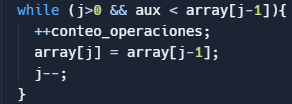
\includegraphics[width=0.8\linewidth]{media/insertionSort.png}
    \caption{Segmento de código colaborativo para la función de \textit{InsertionSort}.}
    \label{fig:insertion}
\end{figure}

\subsection{SelectionSort}

El ordenamiento por selección se considera una forma “natural” de ordenar valores. Consiste en revisar todos los elementos y “seleccionar” el valor más pequeño de la colección para intercambiarlo con el primero. En cada iteración se repite el procedimiento de buscar el menor elemento y colocarlo en la posición correspondiente.\\

La complejidad temporal para este algoritmo es de $O(n^2)$ para todos los casos, ya que incluso para el mejor caso, que es cuando la lista ya se encuentra ordenada, en el ordenamiento siempre se tiene que buscar el elemento mínimo en cada iteración, por lo que hará el mismo número de comparaciones que cuando se encuentra en el peor, por lo que este algoritmo es demasiado ineficiente, quizás funciones para listas pequeñas, ya que de lo contrario, su proceso de ordenamiento es demasiado lento.\\

Para este algoritmo hicimos uso de dos variables para contar las operaciones realizadas por el ordenamiento, las cuales fueron conteo comparaciones al inicio del segundo ciclo \textit{for} y conteo intercambios dentro del \textit{if}, este funcionamiento se puede ver en la Figura 2. Al final se sumaron los dos valores obtenidos de las variables de conteo y gracias a esto determinamos el numero de comparaciones para los diferentes tamaños de listas con respecto a este algoritmo. El segmento de código se muestra a continuación.\\

\begin{figure}[h]
    \centering
    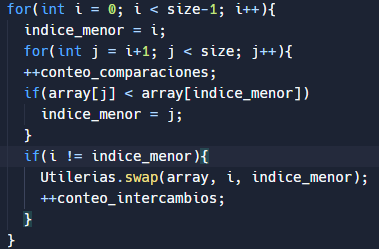
\includegraphics[width=0.8\linewidth]{media/selectionSort.png}
    \caption{Segmento de código del algoritmo \textit{SelectionSort}.}
    \label{fig:selection}
\end{figure}

\subsection{BubbleSort}

En \textit{bubblesort}, de la lista a ordenar se verifica cada dato en relación con el elemento inmediato siguiente, intercambiándose de posición si se encuentra en un orden inverso al requerido.\\

En este algoritmo se implementó una modificación con la variable \textit{k} para que el algoritmo sea sensible a cuando el arreglo ya se encuentra ordenado y no tenga que hacer por consiguinte todas las iteraciones, ésto con el fin de mejorar su complejidad, teniendo que para el mejor de los casos, sea de $O(n)$, y para el caso promedio y el peor de los casos es $O(n^2)$, por lo que también es muy ineficiente para ordenar colecciones de muchos elementos.\\

En est algoritmo, para poder observar su comportamiento en la gráfica generada, contamos con la variable \textit{conteo\_comparaciones} en el segundo \textit{for} las comparaciones realizadas por los elementos de la lista y con la variable conteo intercambios, los correspondientes intercambios realizados en total por el algoritmo después se sumarón los valores de estos contadores. Lo anterior se puede apreciar a continuación, en la Figura 3.

\begin{figure}[h]
    \centering
    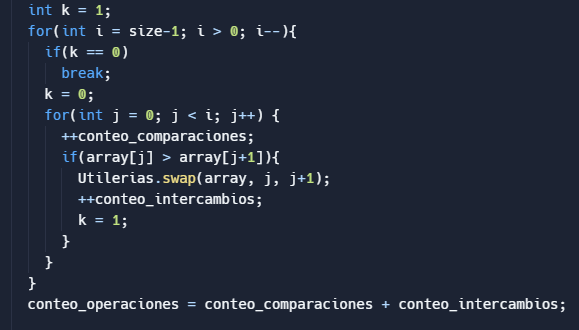
\includegraphics[width=0.8\linewidth]{media/bubble.png}
    \caption{Segmento del código de \textit{BubbleSort}.}
    \label{fig:enter-label}
\end{figure}

\subsection{HeapSort}

HeapSort entra en la lista de los \textit{Algoritmos de Selección}, teniendo la siguiente funcionalidad:

\begin{enumerate}
    \item Convertir colección a ordenar en un \textit{heap}.
    \item En cada iteración, eliminar la raíz (tenemos en cuenta que el proceso de eliminación conlleva la reconstrucción del \textit{Heap}, porque este siempre debe mantener su integridad).
\end{enumerate}

En otras palabras, el algorimo consiste en la construcción de un árbol binario llamado \textit{Heap}, en donde se harán las comparaciones/intercambios con una parte de los elementos de la colección, y finalmente se recorre linealmente todos los elementos al intercambiar con la última posición.\\

Teniendo en cuenta el funcionamiento del algoritmo y entendiendo los procedimientos que realiza, es como logramos determinar que deberían incluirse dos contadores en nuestro código, el primero ubicándolo cuando se construye el \textit{Heap} en el ciclo \textit{for} dentro del método \textit{buildHeap}, y el segundo contador cuando se extraen los elementos y se reconstruye el \textit{heap} hasta que ya no haya más elementos, esto en el método \textit{heapify}.\\  

Cabe resaltar que la complejidad de este algoritmo para todos sus casos es de $O(n \log n)$.

\subsection{QuickSort}

El algoritmo \textit{QuickSort} utiliza el método de intercambio para la realización del reacomodo de los valores y, tomando en cuenta el tiempo y la memoria de una computadora, se termina considerando como uno de los mejores algoritmos de ordenamiento; teniendo tanto para el mejor caso, como para el promedio una complejidad de $O(n \log(n))$ y para su peor caso una complejidad de $O(n^2)$.\\

Este algoritmo emplea como estrategia general:

\begin{enumerate}
    \item Seleccionar un elemento de la colección [pivote].
    \item Verificar este pivote en relación con el resto de los elementos y realizar los intercambios, de tal manera que, aquellos que se encuentren a su izquierda sean menores o igual, y aquellos a la derecha mayores.
    \item Repetir lo anterior en los conjuntos de datos que se generan a la izquierda y a la derecha.
\end{enumerate}

Para la implementación del código en este proyecto, utilizamos el repositorio anteriormente entregado por el profesor durante las prácticas, y las únicas modificaciones que realizamos fueron al momento de inicializar el algoritmo:\\

Implementamos el método: \textit{iniciarQuickSort(int[] array, int low, int high)}, que declara el contador en 0, y de esta manera cuando el algoritmo aplique la recursividad, no se vea afectado el conteo de iteraciones que este realiza, como se puede ver en la Figura 4.\\

\begin{figure}[h]
    \centering
    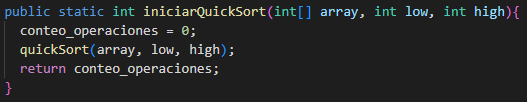
\includegraphics[width=0.8\linewidth]{media/QuickSort_MetodoIniciar.PNG}
    \caption{Código del método: \textit{iniciarQuickSort} en la clase \textit{QuickSort}.}
    \label{fig:iniciarquick}
\end{figure}

El conteo de operaciones se realiza en el método \textit{partition}, dentro de la estructura de selección \textit{if}, y también hace el conteo en la función \textit{quickSort}, para cada llamada recursiva.

\subsection{MergeSort}

El algoritmo de ordenamiento \textit{Merge-sort} sigue la lógica \textit{divide y vencerás} y su funcionamiento radica principalmente en combinar dos listas que ya han sido ordenadas para obtener una respectiva lista ordenada más grande.\\

La estrategia general para este algoritmo es la siguiente:

\begin{enumerate}
    \item Dividir la sublista de \textit{n} elementos en dos sublistas.
    \item Ordenar las dos sublistas utilizando \textit{merge-sort}.
    \item Combinar(intercalar) las dos sublistas ordenadas para obtener la lista ordenada final.
\end{enumerate}

La complejidad de este algoritmo es de $O(n\log(n))$ para todos los casos, lo que lo hace ser rápido con la desventaja de que este algoritmo hace uso de memoria adicional, para tener un arreglo o lista auxiliar para hacer el acomodo de las sublistas que se van generando.\\

Para contar las operaciones realiadas por este algoritmo, se agrego la variable \textit{conteo\_operaciones} dentro de los ciclos \textit{while} por la comparaciones realizadas y dentro del método \textit{mergeSort} por cada vez que se llame a dicho metodo y contar estas operaciones, ésto se puede ver en la Figura 5 y 6.

\begin{figure}[h]
    \centering
    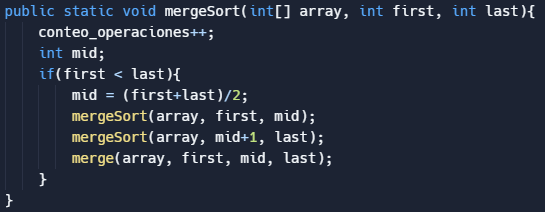
\includegraphics[width=0.5\linewidth]{media/mergesort.png}
    \caption{Segmento de la clase \textit{MergeSort}.}
    \label{fig:merge1}
\end{figure}

\begin{figure}[h]
    \centering
    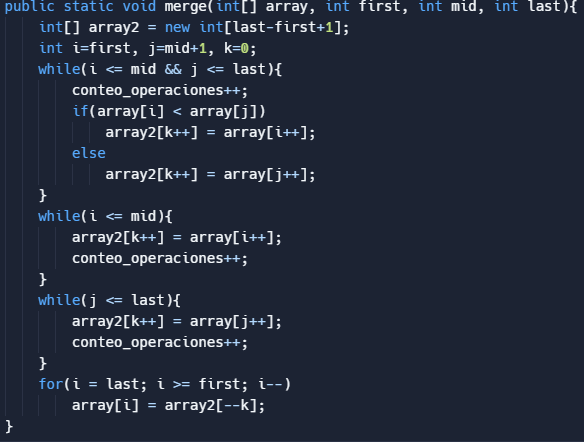
\includegraphics[width=0.5\linewidth]{media/merge.png}
    \caption{Segmento del método \textit{merge} de \textit{MergeSort}.}
    \label{fig:merge2}
\end{figure}

\subsection{CountingSort}

El algoritmo de ordenamiento \textit{CountingSort} no partió de un código brindado, sino que se propuso su implementación en su totalidad.\\

Este ordenamiento destaca en su funcionamiento puesto que requiere una gran cantidad de memoria adicional para ser ejecutado, si bien como se verá más adelante funciona de una menra sumamente rápida, todo este almacenamiento adicional a la colección original lo vuelven una opción no preferida y en algunos casos inviable.

La primera colección adicionarl debe ser del mismo tamaño que la original, en la implementación esta colección se llama \textit{sorted}, la segunda es una colección que debe tener por tamaño el número o rango de elementos que pueden aparecer a ordenar. Por ejemplo, si se quieren ordenar número del uno al cinco, el tamaño de esta coleccón será de cinco, pues los posibles elementos pueden ser 1, 2, 3, 4 ó 5; pero si se quieren ordenar números del 10 al 13, el tamaño de la colección será de 4, pues los elementos se pueden encontrar entre el 10, 11, 12 y 13. En la implementación, dicha colección se llama \textit{counting} y su tamaño está dado por la constante \textit{RANGO} definida en el archivo \textit{Ordenamientos.java} con el valor fijo de 99999.\\

El ordenamiento original divide su funcionamiento en tres etapas muy claras:

\begin{enumerate}
    \item Recorrer toda la lista (arreglo) de atrás para adelante\footnote{Siguiendo la suposición general de que todos los arreglos se quieren ordenar de manera ascendente.} haciendo una primera pasada a todos los elementos de la lista, e incrementando en una unidad su correspondiente espacio en el arreglo \textit{grande} (\textit{counting} para el caso) por cada aparición que tenga dicho elemento.
    
    \item Recorrer ordenadamente el arreglo contador (\textit{counting} para el caso), reescribiendo cada elemento por su suma con todos los elementos anteriores en el arreglo. Ésto permite obtener al instante la posición final de dicho elemento al momento de escribir de nuevo la colección esta vez ordenada.
    
    \item Recorrer una segunda vez la colección original, esta vez de adelante para atrás, y colocar cada elemento en su posición correcta en la colección del mismo tamaño a la original (\textit{sorted} para el caso). Para conocer la posición final se accede al número que tiene relacionado en el arreglo contador (obtenido en el paso dos) decrementado en uno, si la posición no está vacía significa que otro mismo elemento como él ocupa el espacio y decrementa otra unidad la posición hasta encontrar finalmente un espacio vacío. Finalmente copia el arreglo ordenado en el original.
\end{enumerate}

Estos tres puntos del funcionamiento, tal como se describieron son implementados cada uno en un método específico:

\begin{enumerate}
    \item count(int[] array, int[] counting, int size)
    \item suma(int[] counting, int numElements)
    \item sort(int[] array, int[] sorted, int[] counting, int size)
\end{enumerate}

\subsection{RadixSort}

El funcionamiento de \textit{RadixSort}, al igual que \textit{CountingSort}, es un tanto alternativo al resto de los presentados, pues no se basan en las operaciones de comparación e intercambio sino de una manera más \textit{innovadora}.\\

La lógica original de este ordenamiento consiste en tomar cada dígito de cada elemento en la colección y, dependiendo de su valor, agregarlo a una cola (\textit{queue}) con el valor asignado, es decir, que existe una cola para cada número natural (0, 1, 2, 3, 4, 5, 6, 7, 8, 9). Una vez encolados todos los elementos, se deben desencolar todas las colas de manera ordenada, es decir, primero la del uno, luego la del dos, luego la del tres... Esta operación se repetirá para todos los dígitos de todos los elementos en la colección.\\

De nuevo, este ordenamiento aunque sí destaca por la velocidad temporal al momento de trabajar con grandes volúmenes de información, tiene también un alto costo en materia de almacenamiento adicional equivalente al doble de la colección original, pues en cada iteración el contenido total del arreglo original será repartido en todas las colas, que a su vez reescribirán la colección original.\\

La implementación para este proyecto inicia con la declaración de las diez colas, y obtiene el número de digítos del elemento más grande en la lista mediante la invocación a las funciones \textit{getMax} y \textit{getIterations}\footnote{Ésto permite que el programa funcione correctamente ante cualquier arreglo de entrada, siempre que sea del mismo tipo, sin importar el tamaño de los números contenidos en el arreglo.}.

El algoritmo funciona en un ciclo \textit{for} para cada dígito, en el que recorre cada vez la lista y obtiene el dígito correspondiente de los números (haciendo división entre 10, 100, 1000 y así sucesivamente) y añade el dígito a la cola que le corresponde. Finalmente reescribe el arreglo original vaciando el contenido de las colas en orden. El contador se incrementa en el segundo ciclo \textit{for}, cuando recorre \textit{iteraciones} veces los elementos del arreglo. Para este caso el número más grande es 99999, por lo que el número máximo de dígitos será de cinco, y posteriormente en la gráfica se debería de ver su gráfica como \textit{5n}, siendo \textit{n} el número del tamaño del arreglo.

\subsection{PancakeSort}

Para este proyecto, se decidió agregar el algoritmo de ordenamiento PancakeSort.\\

PancakeSort es un algortimo de ordenamiento, en el cual su funcionamiento se asemeja a la actividad de voltear hotcakes o panqueques, pues el procedimiento de este algoritmo consiste en voltear segmentos de lista, tal y como se haria con una porción de panqueques.\\

Este algoritmo, encuentra al elemento de mayor valor en la lista y posteriormente lo coloca en su posición correspondiente mediante operaciones de volteo. El proceso anterior se repite con los elementos mayores en la lista, hasta que se ordene en su totalidad dicha colección.\\

Es importante mencionar, que para este algoritmo, a diferencia de otros donde se busca hacer el menor número de comparaciones, en este la operación principal es el volteo de los segmentos de lista.\cite{ord-panq}\\

Para llevar a cabo la implementación de este algoritmo, con ayuda del material de apoyo obtenido de fuentes de internet\cite{gfg-2023}, encontramos un código del algoritmo en el lenguaje de programación C++ y analizando su estructura, lo adaptamos a nuestro proyecto realizado en el lenguaje de programación Java, satisfaciendo nuestras necesidades, en referencia al ordenamiento de listas de diferentes tamaños.\\

Respecto a la complejidad espacial de este algoritmo, esta se denota por $O(1)$ ya que no ocupa memoria adicional, sin embargo, en lo que refiere a su complejidad temporal, para el mejor de los casos es $O(n)$, pero para el caso promedio y el peor de los casos, la complejidad es de O($n^2$), pues el algoritmo en un proceso de ordenación de una determinada lista, puede llegar a requerir realizar hasta dos operaciones de volteo por elemento, lo que lo hace ser muy lento para ordenar listas de tamaños de elementos muy grandes y en consecuencia se vuelve ineficiente su uso.\cite{gfg-2023}\\

Una manera fácil de entender el funcionamiento general de este algoritmo la ofrece el video \textit{Pancake sort algorithm, visualization with VTK} (Mario Storti, 2009)\cite{video-vtk}.

Más adelante, gracias a la correspondiente grafica generada entre los algoritmos de ordenamiento de complejidad cuadrada, pudimos apreciar su correspondiente comportamiento para listas de tamaños muy grandes, así como ver que algoritmos son mejores o peores en relación a PancakeSort.\\

Para este algoritmo, incrementando la variable \textit{conteo\_operaciones} se contaron sus correspondientes operaciones realizadas como se muesta en la Figura 7, que es donde se realizan los respectivos volteos del algoritmo.

\begin{figure}[h]
    \centering
    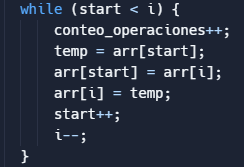
\includegraphics[width=0.8\linewidth]{media/segmento_pancake.png}
    \caption{Segmento de la clase \textit{PancakeSort}.}
    \label{fig:seg-pancake}
\end{figure}

\section{Análisis de resultados}

Al realizar el análisis de complejidad en la reiterada ejecución de estos algoritmos de ordenamiento, se buscan ciertas formas específicas en los trazos que deberían tener. Al momento de decidir qué algoritmos graficar juntos se tomó la decisión de poner en el mismo cuadro aquellas que tengan un comportamiento téorico similar, de manera que:

\begin{itemize}
    \item $\mathbf{O(n^2)}$ \\\textit{InsertionSort}, \textit{SelectionSort}, \textit{BubbleSort}, \textit{PancakeSort}.
    \item $\mathbf{O(n\log(n))}$ \\\textit{QuickSort}, \textit{HeapSort}, \textit{MergeSort}.
    \item $\mathbf{O(n+k) \ \& \ O(n+k)}$ \\\textit{CountingSort} y \textit{RadixSort}.
\end{itemize}

Se decidió añadir, junto a los trazos de cada ordenamiento, en su respectivo cuadro un trazo extra de control, en el cual se muestran la gráfica cuya forma debe ser esperada: $y=x^2$, $y=x\log(x)$ y $y=x$ respectivamente. De manera adicional, hizo uso de la aplicación \textit{GeoGebra} para tener también a la mano las gráficas correspondientes y la forma en la que idealmente se deberían de ver, la primera y tercera se muestran en la Figura 8 y Figura 9, respectivamente.

\begin{figure}[H]
    \centering
    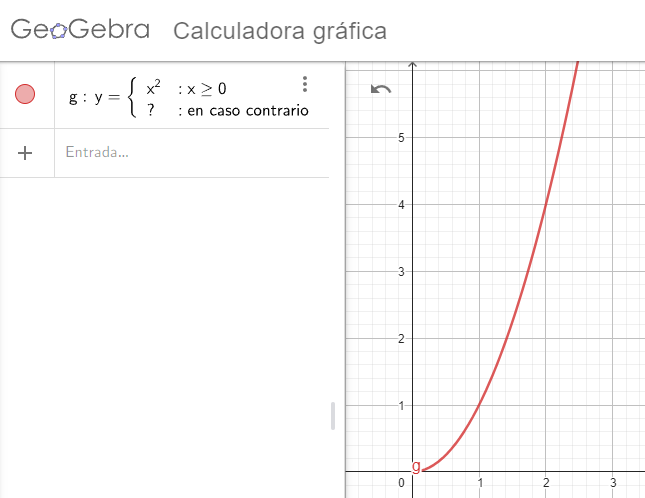
\includegraphics[width=.9\textwidth]{media/semiparabola-geogebra.png}
    \caption{Gráfica teórica para $y=x^2$ obtenida en \textit{GeoGebra}.\cite{geogebra}}
    \label{fig:semiparabola-geogebra}
\end{figure}

\begin{figure}[H]
    \centering
    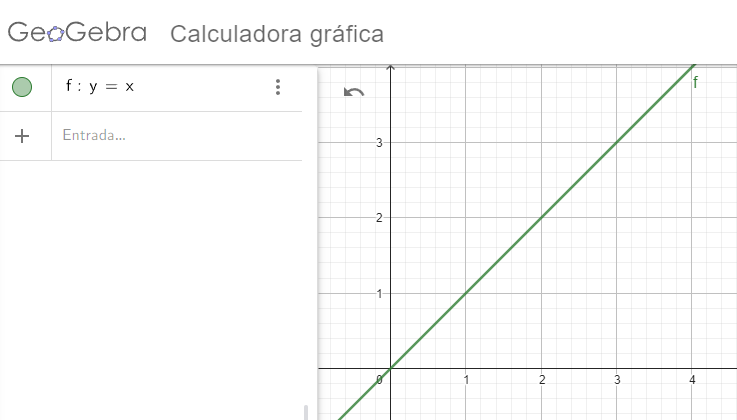
\includegraphics[width=.9\textwidth]{media/identidad-geogebra.png}
    \caption{Gráfica teórica para $y=x$ obtenida en \textit{GeoGebra}.\cite{geogebra}}
    \label{fig:identidad-geogebra}
\end{figure}

Ante la incertidumbre de cómo se debe de generar la gráfica de $n\log(n)$, del mismo modo que en las gráficas anteriores, se hizo en el software de \textit{GeoGebra} la gráfica buscada para la referencia precisa de cómo se debería de ver, dicha imagen se encuentra en la Figura 10.

\begin{figure}[h]
    \centering
    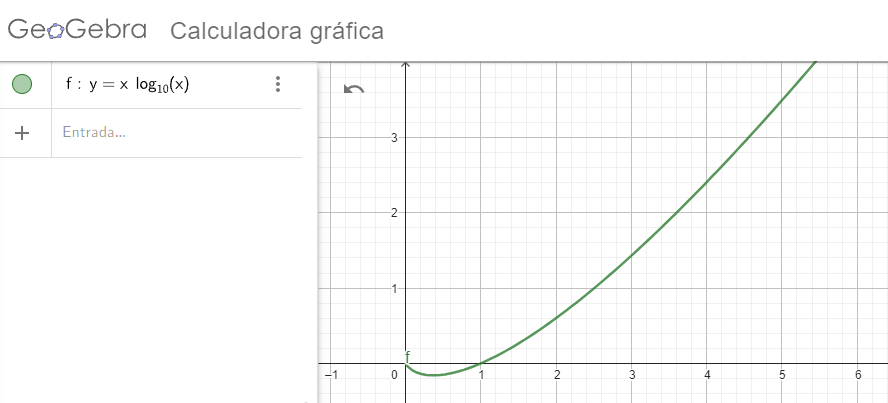
\includegraphics[width=.9\textwidth]{media/nlogn-geogebra.png}
    \caption{Gráfica teórica para $y=xlog(x)$ obtenida en \textit{GeoGebra}.\cite{geogebra}}
    \label{fig:nlogn-geogebra}
\end{figure}

Y teniendo en mente ahora la idea de cómo se debería de ver, se ejecutó en el archivo \textit{GraficarLogaritmo.py} la misma gráfica desde a partir de un centésimo y hasta cinco mil, como se puede ver en la Figura 11.

\begin{figure}[H]
    \centering
    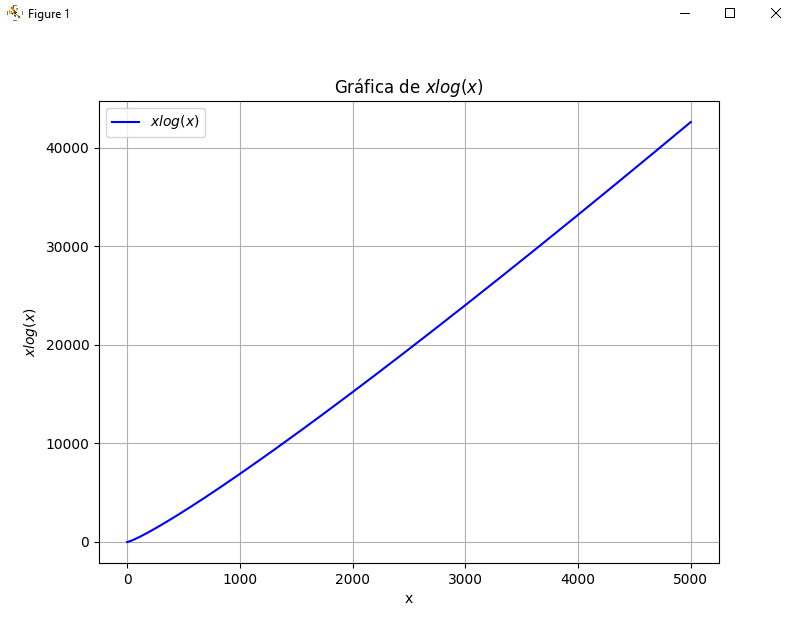
\includegraphics[width=.8\textwidth]{media/xlogx_desde_01.png}
    \caption{Gráfica comparativa para $y=xlog(x)$ obtenida en \textit{GraficarLogaritmo.py} desde un valor mínimo de 0.01.}
    \label{fig:nlogn-python1}
\end{figure}

Y teniendo la muestra de lo que se debería esperar ver en las gráficas capaces de realizar de primera mano, se hizo una ejecución donde el tamaño de entrada fuera cinco mil, ésto con el propósito de que la entrada (y por tanto el eje x) de ambas gráficas pudiera coincidir. El resultado se muestra en la Figura 12.

\begin{figure}[h]
    \centering
    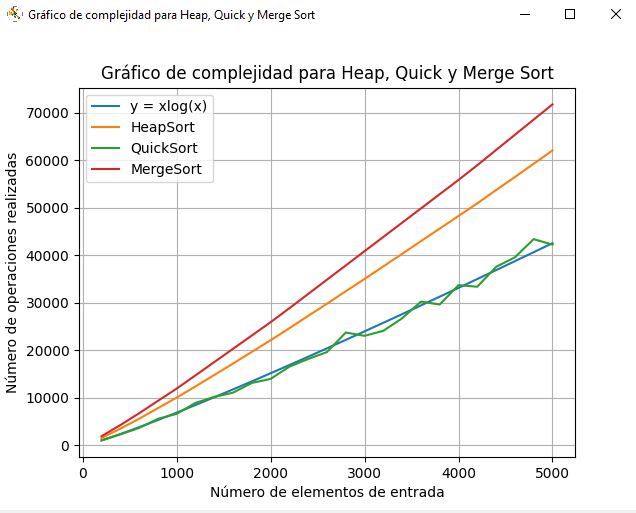
\includegraphics[width=.8\textwidth]{media/nlogn_en_5000.png}
    \caption{Gráfica obtenida experimentalmente para $y=xlog(x)$ obtenida en \textit{Graficar.py} con una entrada de cinco mil.}
    \label{fig:nlogn-python2}
\end{figure}

Dándose cuenta de que, aún así, la gráfica obtenida al realizar los ordenamientos difiere levente de lo esperado, aunque este hecho pudo ser fácil de explicar al contrastar el tamaño mínimo de entrada, en la gráfica de muestra se tiene como valor mínimo en el eje x uno muy pequeño, de 0.01, mientras que la entrada mínima del programa es de 200, intervalo decidido así por conveniencia en los distintos tamaños. Al darle una entrada a \textit{GraficarLogaritmo.py} igual a la del programa principal, de 200, se obtuvo la gráfica que se ve en la Figura 13.

\begin{figure}[h]
    \centering
    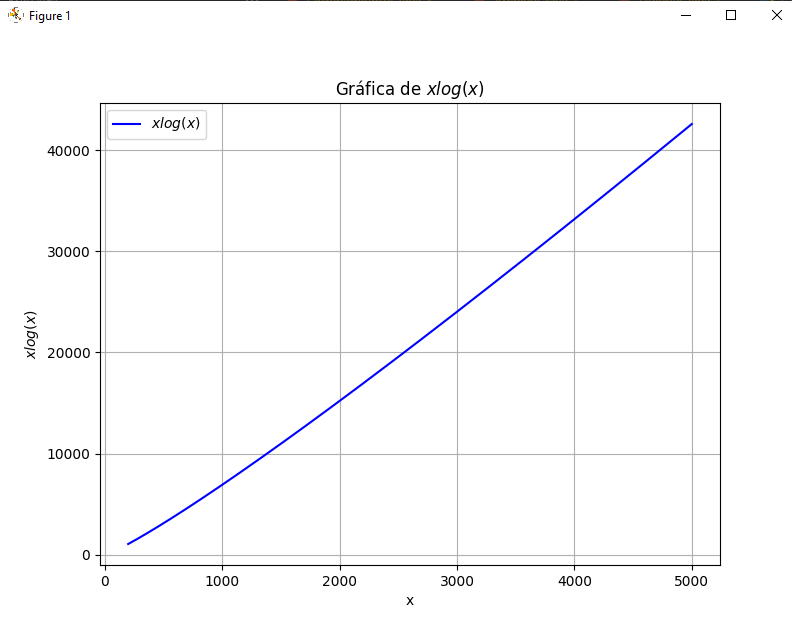
\includegraphics[width=.8\textwidth]{media/xlogx_desde_200.png}
    \caption{Gráfica comparativa para $y=xlog(x)$ obtenida en \textit{GraficarLogaritmo.py} desde un valor mínimo de 200.}
    \label{fig:nlogn-python3}
\end{figure}

Es así como se logró ganar la fiabilidad de la correcta graficación el programa desarrollado en Python para mostrar las gráficas, siendo que, bajo las mismas condiciones, ambas gráficas se asemejan de una manera en la que se ven casi exactamente iguales, indicando que el trazo en el gráfico de ordenamientos de control ($y=xlog(x)$) es correcto en su comportamiento y capaz de ser un punto de control para el trazo obtenido en la imagen de las gráficas con los volúmenes de información más grandes realizados.\\

En la siguiente gráfica (\textit{Figura 14}) se muestran los Algoritmos de Ordenamiento de \textit{Insertion}, \textit{Selection}, \textit{Bubble} y \textit{Pancake}. Estos algortimos se recopilaron en una misma gráfica porque en el caso promedio todos tienen una complejidad $O(n^2)$.\\

Para la construcción de esta gráfica consideramos que se ordenaron 20,000 elementos en cada uno de los algoritmos, y podemos apreciar que con esta cantidad de elementos se llegó a realizar en el peor algoritmo (BubbleSort) hasta $3 \times 10^8$ operaciones, mientras que el mejor algoritmo (InsertionSort) realizó $1 \times 10^8$ operaciones. \\

Cabe destacar que en la gráfica se colocó el valor teorico $y = x^2$ para tenerlo como referencia y así poder hacer la comparación con los resultados de los algoritmos. De esta manera, al tener una similitud en la graficicación entre el valor teorico y los resultados de los algoritmos, podemos afirmar que todos cumplen con la complejidad $O(n^2)$.\\

\begin{figure}[h]
    \centering
    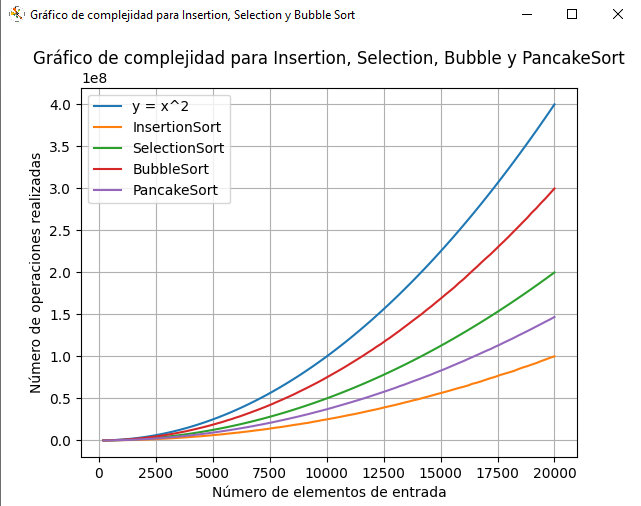
\includegraphics[width=1\textwidth]{media/graficaA_20k.png}
    \caption{Gráfica de ordenamientos con complejidad $O(n^2)$ para una entrada de veinte mil elementos.}
    \label{fig:grafA_20k}
\end{figure}

En esta gráfica al igual que en la anterior se muestra el comportamiento de los algoritmos Insertion, Selection, Buble y Pancaker sort, pero en este caso, ordenando listas de hasta un tamaño 100,000 elementos, ésto con la finalidad de poder corroborar para listas de tamaños mucho más grandes, qué algoritmo es el que termina siendo más eficiente o ineficiente en su defecto, visualizando cuál tarda más en ordenar la lista según el tamaño.\\

Como se puede apreciar, de todos los algoritmos, según sus correspondientes comportamientos, Bubble es el ordenamiento que más se aproxima al comportamiento teórico de $O(n^2)$ y la que menos se parece a dicho comportamiento teórico es la de insertion, por lo que comparando a estos cuatro algoritmos, posiblemente el mejor de ellos es InsertionSort. Figura 15.

\begin{figure}[h]
    \centering
    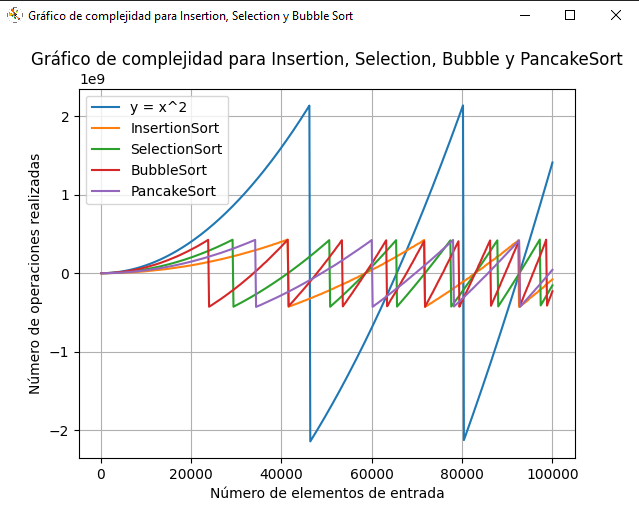
\includegraphics[width=1\textwidth]{media/graficaA_100k.png}
    \caption{Gráfica de ordenamientos con complejidad $O(n^2)$ para una entrada de cin mil elementos.}
    \label{fig:grafA_100k}
\end{figure}

Para la siguiente gráfica, se presentan los respectivos comportamientos de los algoritmos Heap, Quick y Merge sort, para listas que van hasta un tamaño de 20,000 elementos. Como se puede observar, estos algorimos tenen un comportamiento con complejidad $O(n\log(n))$, siendo quick, la que se comporta mejor de las tres y, en consecuencia, es más rápida a la hora de realizar los ordenamientos.\\
Por otro lado, primero se graficó probando con esta cantidad de elementos, para posteriormente visualizar qué tanto difiere o no con listas de tamaños aun más grandes y así verificar qué algoritmo es el mejor.

\begin{figure}[h]
    \centering
    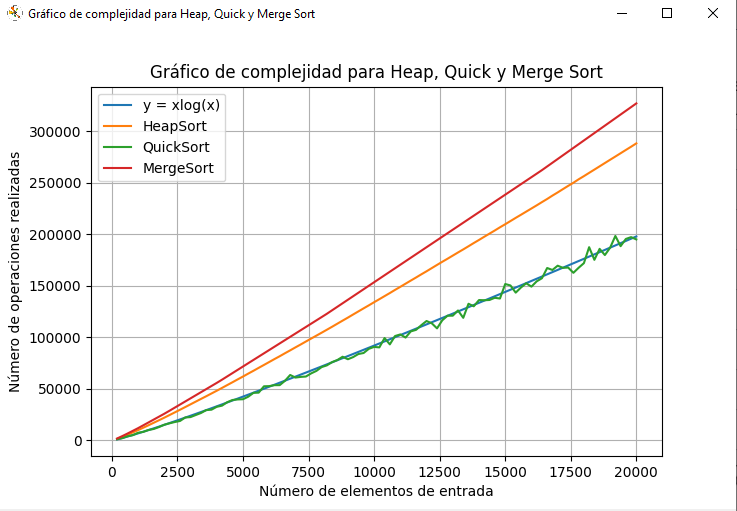
\includegraphics[width=1\textwidth]{media/graficaB_20k.png}
    \caption{Gráfica de ordenamientos con complejidad $O(n\log(n))$ para una entrada de veinte mil elementos.}
    \label{fig:grafB_20k}
\end{figure}

Continuamos con la gráfica que compara los algoritmos: Heap, Quick y Merge (\textit{Figura 17}). En este caso, se realiza un ordenamiento de 100,000 elementos, siendo el mejor algoritmo QuickSort, que realiza un aproximado de $1.2 \times 10^6$ operaciones, seguido de HeapSort que realiza un aproximado de $1.6 \times 10^6$ operaciones, y finalmente como peor algoritmo de esta comparación, tenemos a MergeSort que realiza aproximadamente $1.8 \times 10^6$ operaciones.\\

Recordamos que para el caso promedio de estos algoritmos, su complejidad es de $O(n\log(n))$.\\

\begin{figure}[h]
    \centering
    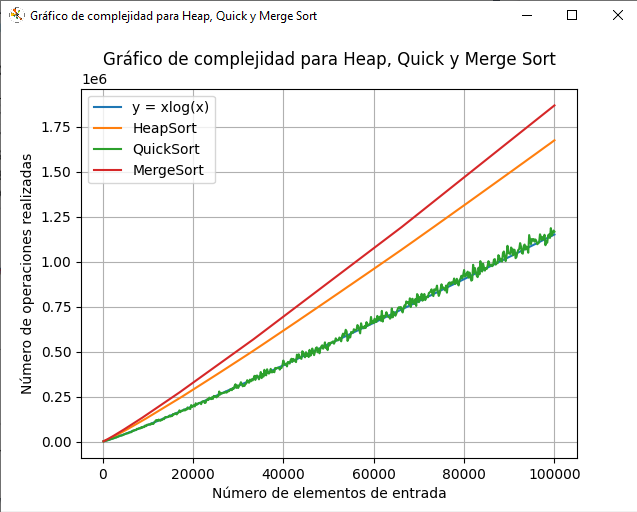
\includegraphics[width=1\textwidth]{media/graficaB_100k.png}
    \caption{Gráfica de ordenamientos con complejidad $O(n\log(n))$ para una entrada de cien mil elementos.}
    \label{fig:grafB_100k}
\end{figure}

Para esta gráfica, se presentan los algoritmos Couting y Radix sort, ordenando listas de elementos de hasta tamaño 20,000. Como se puede visualizar, se cumple con su compleidad que es de $O(n+k)$ y $O(nk)$ respectivamente.\\

Se puede visualizar que ambas siguen su correspondiente comportamiento esperado y se parecen a la gráfica teórica. Otro punto importante a destacar es que se puede observa cómo es que Radix es peor que Couting, pues el número de operaciones que realiza el primero es mucho mayor que el de couting, lo que nos puede ayudar a entender que en este caso, termina siendo mejor CoutingSort.\\

Se optó por realizar esta gráfica para primero ver su comportamiento con una lista de elementos de tamaño menor, para posteriormente apreciar como se comportan los algoritmos con listas mas grandes. Figura 18.

\begin{figure}[h]
    \centering
    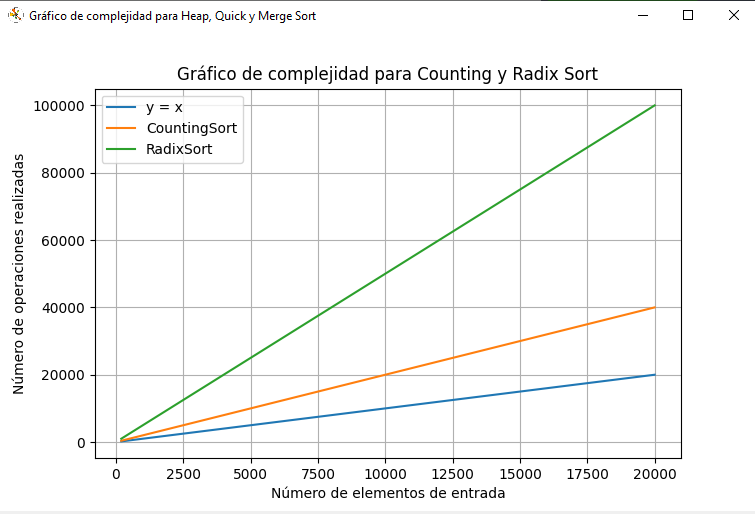
\includegraphics[width=1\textwidth]{media/graficaC_20k.png}
    \caption{Gráfica de ordenamientos con complejidad  $O(n+k)$ y $O(nk)$ para una entrada de veinte mil elementos.}
    \label{fig:grafC_20k}
\end{figure}

Ahora la gráfica (\textit{Figura 19}) que de igual manera compara los algoritmos de Countig y Radix Sort, ordenan 100,000 elementos. Y el resultado que se muestra nos hace corroborar que por más elementos que ordenen siempre será CountingSort el algoritmo más rápido, ya que este realizó 200,000 operaciones, mientras que RadixSort realizó 500,000 operaciones. \\

Cabe recodar que estos algoritmos tienen una complejidad en su caso promedio de $O(n+k)$, que de igual manera se muestra como referencia en la gráfica de color azul.  

\begin{figure}[h]
    \centering
    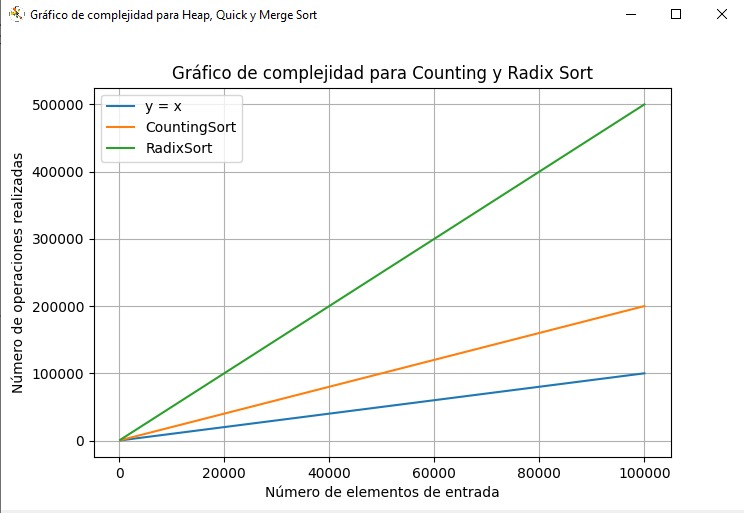
\includegraphics[width=1\textwidth]{media/graficaC_100k.jpg}
    \caption{Gráfica de ordenamientos con complejidad $O(n+k)$ y $O(nk)$ para una entrada de cien mil elementos.}
    \label{fig:grafC_100k}
\end{figure}

En la gráfica actual, se junto a todos los algoritmos estudiados en el proyecto, realizandoles pruebas de ordenamiento para listas de hasta 20,000 elementos. Lo anterior fue con motivo a poder observar en general a todas las gráficas y asi que algoritmo es más eficiente.\\

Como se puede apreciar, al variar sus complejidades, todos los que no sean O($n^2$) prácticamente no es posible verlos y únicamente se aprecian los que sí pertenezcan a dicha complejidad, por lo que podemos ver que, comparando a todos los algoritmos, aquellos que se pueden visualizar su complejidad cuadratica son los peores, tal es el caso de bubble, selection, pancake e insertion sort. Figura 20.

\begin{figure}[h]
    \centering
    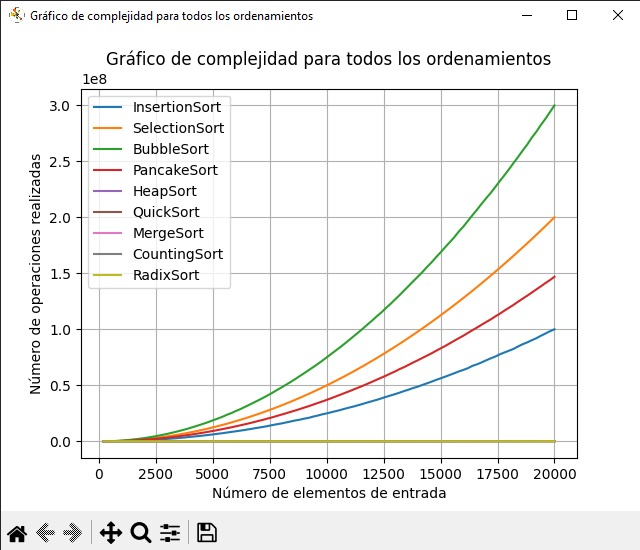
\includegraphics[width=1\textwidth]{media/graficaD_20k.jpg}
    \caption{Gráfica de todos los ordenamientos para una entrada de veinte mil elementos.}
    \label{fig:grafD_20k}
\end{figure}

En esta gráfica (\textit{Figura 21}), también tenemos todos los algoritmos analizados en este proyecto, solo que en esta ocasión, el número de elementos a ordenar es de 100,000.\\

Obvervando lo que sucede con cada algoritmo, podemos notar que los algoritmos Counting, Merge, Quick, y Heap se encuentran ocultos, ya que están por debajo de la graficación de RadixSort. Esto nos muestra la gran diferencia que hay entre los algoritmos de complejidad $O(n^2)$ y, los de complejidad $O(n\log(n))$ y $O(n+k)$. Siendo mejor los algoritmos: Radix, Counting, Merge, Quick, y Heap. Para el ordenamiento de elementos muy grandes. Aunque, hay que recordar que los algoritmos de Counting y Radix por más eficientes que sean en el tiempo para el ordenamiento de elementos, utilizan mucha memoria. 

\begin{figure}[h]
    \centering
    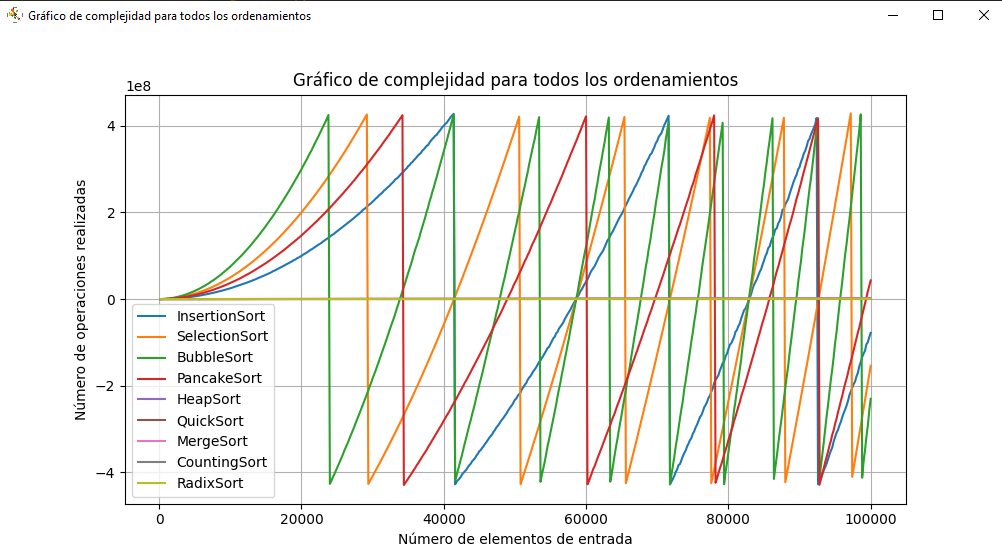
\includegraphics[width=1\textwidth]{media/graficaD_100k.png}
    \caption{Gráfica de todos los ordenamientos para una entrada de cien mil elementos.}
    \label{fig:grafD_100k}
\end{figure}

En la presente gráfica, se comparan los algoritmos de complejidad $O(nlog(n))$ Quick, Merge y Heap sort, junto con los algoritmos Couting y Radix sort, de complejidad $O(n+k)$ y $O(nk)$ respectivamente. En este caso, se les encomendó ordenar listas de hasta tamaño 20,000. La finalidad de esta gráfica es observar inicialmente cómo se comportan los algoritmos al ordenar primero hasta la cantidad mencionada de elementos.\\

Lo que se puede observar tras realizar el correspondiente análisis de los algoritmos, es que quick es mejor que sus semejantes en comlejidad pero es superado por couting y radix, pues estos dos últimos realizan menos operaciones, pero no hay que olvidar que requieren del uso de memoria adicional para ser utilizados. Figura 22.

\begin{figure}[h]
    \centering
    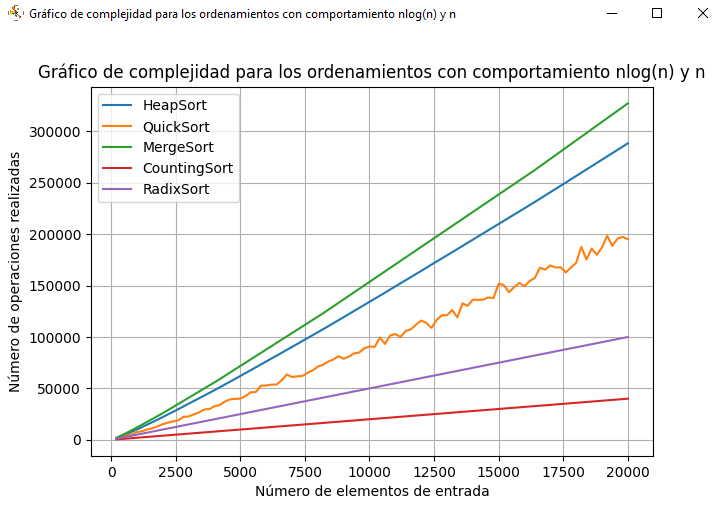
\includegraphics[width=1\textwidth]{media/graficaE_20k.png}
    \caption{Gráfica de todos los ordenamientos que no tienen una complejidad $O(n^2)$ para una entrada de veinte mil elementos.}
    \label{fig:grafE_20k}
\end{figure}

Finalmete, la siguiente gráfica (\textit{Figura 23}), nos muestra la comparación de los algoritmos: Heap, Quick, Merge, Counting y Radix. Que corresponden a una complejidad en sus casos promedios de $O(n\log(n))$ y $O(n+k)$, respectivamente. \\

Podemos notar que el mejor de estos algoritmos es CountingSort, realizando un aproximado de $0.3 \times 10^6$ operaciones, después tenemos a RadixSort que realiza un aproximado de $0.5 \times 10^6$ operaciones. Estos dos algoritmos cumplen con una complejidad de $O(n+k)$. \\

Posteriomente, tenemos los algoritmos de complejidad $O(n\log(n))$, siendo el 3er mejor algortmo QuickSort, después le sigue HeapSort, y al final tenemos a MergeSort que sería el peor algoritmo de estas comparaciones realizando un aproximado de $1.80 \times 10^6$ operaciones.\\

De esta manera concluimos que los algoritmos de complejidad $O(n+k)$ son los mejores ordenando elementos en cuestión de tiempo, auqnue su desventaja es el uso excesivo de memoria.\\ 

\begin{figure}[h]
    \centering
    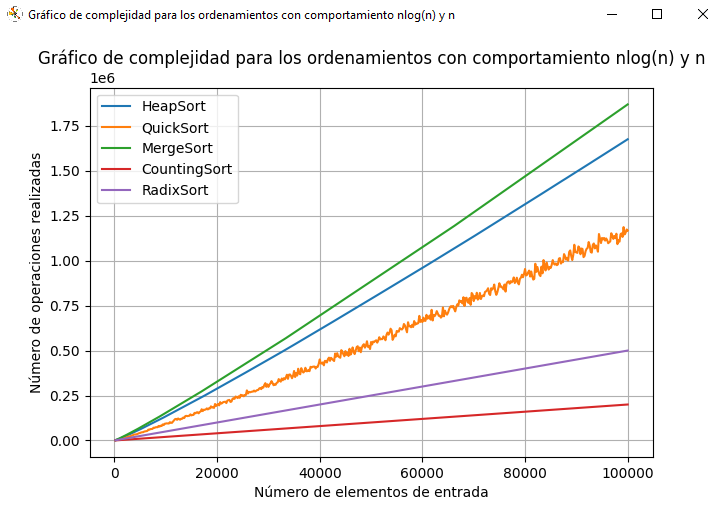
\includegraphics[width=1\textwidth]{media/graficaE_100k.png}
    \caption{Gráfica de todos los ordenamientos que no tienen una complejidad $O(n^2)$ para una entrada de cien mil elementos.}
    \label{fig:grafE_100k}
\end{figure}

Después de haber probado todos los algoritmos de ordenamiento del proyecto, así como haber analizado el comportamiento de sus graficas generadas, pudimos observar que los algoritmos \textit{insertion}, \textit{selection}, \textit{bubble} y \textit{pancake}, al ser algoritmos de complejidad $O(n^2)$, son muy lentos al realizar los ordenamientos. Por su parte, \textit{couting} y \textit{radix}, de complejidad $O(n+k)$ y $O(nk)$ que por el factor espacial su complejidad temporal termina siendo lineal, por ese factor del espacio terminan siendo menos eficientes y más costosos computacionalmente.\\

Finalmente los algoritmos de mayor eficiencia fuerón \textit{heapsort}, \textit{quicksort} y \textit{mergesort}, por su complejidad $O(n\log(n))$, son los más veloces y entre estos, según la gráfica obtenida, el mejor fue \textit{quicksort}, por lo que de todos los algoritmos analizados este fue el más eficiente en cuestión de tiempo, sin embargo, a pesar de que consideramos que pusimos a contar las operaciones de este algoritmo en el lugar correcto del código, por alguna razón el comportamiento de la gráfica tiene unas ciertas variaciones y sinceramente desconocemos porque se dio este comportamiento. Aunque podemos suponer que tal vez se dio debido a algún ligero error en el código de la implementación de este algoritmo o tal vez no logramos identificar de manera correcta en su totalidad las partes del código donde se debían contar las operaciones, pues el comportamiento de la gráfica es demasiado similar al esperado.\\

Tras lo anterior y todo el análisis realizado de los algoritmos comparados y estudiados en el proyecto, consideramos que con respecto al cuestionamiento de cuál es mejor, \textit{quicksort} o \textit{heapsort}, \textit{quicksort} termina siendo más rapido que heap, pues en la grafica, este algoritmo tiene un mejor comportamiento y esto posiblemente se debe a que quick realiza intercambios mas eficientes y \textit{heap} termina haciendo un numero mayor de comparaciones e intercambios.\\

Recopilando los resultados obtenidos por las gráficas de las Figuras 20 y 23, y basándonos en los análisis de complejidad de ellas, podemos enumerar nuevamente todos los ordenamientos trabajados en el orden de eficacia, siendo el número uno el más eficiente de los nueve, y el número nueve el menos eficiente de todos.

\begin{enumerate}
    \item CountingSort.
    \item RadixSort.
    \item QuickSort.
    \item HeapSort.
    \item MergeSort.
    \item InsertionSort.
    \item PancakeSort.
    \item SelectionSort.
    \item BubbleSort.
\end{enumerate}

Sin embargo no debemos de perder de vista el hecho de que todo el análisis hecho para estos ordenamientos presenta únicamente el análisis \textbf{temporal}, y para el caso de los ordenamientos \textit{RadixSort} y \textit{CountingSort} se debe de considerar seriamente también el análisis \textbf{espacial} que no aborda esta investigación por lo que, enumerando nuevamente los ordenamientos bajo el mismo criterio, pero sin considerar a estos dos algormitmos por las razones dichas, tenemos que:

\begin{enumerate}
    \item QuickSort.
    \item HeapSort.
    \item MergeSort.
    \item InsertionSort.
    \item PancakeSort.
    \item SelectionSort.
    \item BubbleSort.
\end{enumerate}

De nuevo, si limitamos esta lista a únicamente los ordenamientos abordados a lo largo de la impartición del tema en la asignatura, la lista queda de la siguiente forma:

\begin{enumerate}
    \item QuickSort.
    \item HeapSort.
    \item MergeSort.
    \item InsertionSort.
    \item SelectionSort.
    \item BubbleSort.
\end{enumerate}

Es así como se puede ver claramente que el ordenamiento de \textit{QuickSort} es el más veloz de todos, seguido de \textit{HeapSort}, y en tercer lugar el último de aquellos de complejidad $O(n\log(n))$ \textit{MergeSort}. Siendo que, como se vió en la Figura 15, cuando se escala el tamaño de la entrada, los algoritmos de complejidad $O(n^2)$ se vuelven inviables de utilizar. Aún así, de entra éstos últimos el más eficiente resulta ser \textit{InsertionSort}, seguido de \textit{PancakeSort}, \textit{SelectionSort} y, como el peor de todos los ordenamientos presentados, \textit{BubbleSort}.

Un comentario extra a lo dicho sobre el análisis es que, la ejecución del programa con la entrada de diez mil tardó exactamente diecisiete horas y veinte minutos. A veces es difícil que podamos interpretar por nuestra cuenta los datos obtenidos experimentalmente, en especial cuando se trabajan con tantos datos. De las diecisiete horas y veinte minutos, los primeros cuatro algoritmos en realizarse (los de complejidad $O(n^2)$) tardaron diecisiete horas exactas en ejecutarse, los veinte minutos restantes fue lo que tardaron el resto de algoritmos en ejecutarse. Este comportamiento refuerza lo visto en al Figura 20.

\section{Conclusiones}

\subsection{Cabrera Rojas Oscar}

Los objetivos se cumplieron satisfactoriamente, al alumno implementó, recopiló e investigó de manera correcta distintos algoritmos de ordenamiento para el lenguaje de programación Java, e identificó correctamente los lugares del código en los que se realizan operaciones de inserción, comparación, intercambio e intercalación mediante el uso variables contadoras cuyo fin es contar el número de operaciones que necesitó, en cada ejecución, para cumplir su cometido; siendo capaz de desarrollar un programa principal cuyo funcionamiento ejecuta el número de veces deseado por el usuario cada uno de los ordenamientos cinco veces para obtener un valor promedio y automatizó el proceso de construcción de tablas y graficación de resultados para analizar satisfactoriamente lo sucedido en cada caso, permitiéndole manejar grandes volúmenes de información de manera fácil y eficaz.\\

Con todo ésto creo el entorno necesario para analizar y observar la complejidad temporal computacional de cada algoritmo de ordenamiento, evidenciando las principales diferencias entre cada uno de ellos y obteniendo una concordancia directa con la complejidad teórica en cada caso.\\

Finalmente concluyó que el algoritmo más eficiente es \textit{Countingsort} a costa de una cantidad considerable de memoria adicional por colecciones adicionales a la original, y enfocado meramente en el análisis temporal, que fue el abordado en esta investigación, el algoritmo de ordenamiento más eficiente es \textit{QuickSort}.\\

Colaboró y se organizó con los integrantes de su equipo para la delegación de tareas, creando un flujo de trabajo acorde, y en el que la delegación de tareas fue adecuada y afin a las aptitudes de cada integrante, logrando una participación activa en el tanscurso del desarrollo del proyecto; la resolución de problemas fue abordada de manera democrática y adecuada para todos los problemas. Las reuniones fueron programadas y organizadas enfocadas en sus objetivos para maximizar el tiempo invertido.\\

El alumno requirió de conocimientos intermedios sobre el lenguaje de programación Java como medio y herramienta para un fin más que como un lenguaje orientado a objetos; conocimientos en profundidad sobre los distintos algoritmos de ordenamiento y en la teoría de lo que son las operaciones de ordenamiento, las necesidades y limitaciones, así como del compromiso espacio-temporal. Adicionalmente también requirió de conocimientos superficiales en el uso general de archivos para su escritura / lectura, y del lenguaje de programación Python, enfocado a la creación de gráficos.\\

La creación de este proyecto y la conjunción de esfuerzos como actividades realizadas tal como se planteó fue el cierre perfecto para el tema de ordenamientos, obligando al alumno a entenderlos en su totalidad para ser capaz de implementarlos, y reforzando el entendimiento que tiene sobre ellos al ver la consecuecia gráfica de lo realizado. Sin duda alguna ayudó al estudiante a comprender mejor el tema.

\subsection{Chavez Marquez Sergio Antonio}

Al termino de este proyecto, se cumple con todos los requisitos obligatorios estipulados en el archivo \textit{“Proyecto 1. Ordenamiento”}: Códigos, video explicativo, documentación y el trabajo escrito, que es el presente documento.\\

Respecto al objetivo, considero que se cumple con éxito, ya que este proyecto además de cumplir con la contabilización de datos en cada algoritmo, se muestran las tablas de los valores promedio comparados y el tiempo que le tomo a cada algoritmo ejecutar los ordenamientos (tomando en cuenta que el tiempo fue medido con el conteo de las iteraciones en cada algoritmo). Estos datos finales que nos proyecta el programa nos permitieron hacer la construcción de las gráficas para la posterior comparación de complejidad entre los algoritmos.\\

Cabe resaltar que el proyecto viene acompañado de unos archivos Python que son auxiliares en la construcción de gráficas, y que nos permitieron realizar un mayor número de pruebas para la comparación del funcionamiento del programa en distintos tamaños de la lista (arreglo). Es decir, que el usuario no tiene la necesidad de estar registrado las iteraciones que realiza cada algoritmo, automáticamente el programa crea archivos “.txt” que almacenan esta información, y que son utilizados al ejecutar el archivo “Graficar.py”.\\

En relación a los resultados obtenidos, considero que todos los algoritmos demostraron la complejidad de la que ya teniamos noción en las clases teoricas (para el caso promedio), aunque se presentó una única ``anomalia'' en la graficación de QuickSort, pero al final lo consideramos como aceptable. De esta manera, logramos ver que este algoritmo termina siendo el mejor de todos, ``ganando'' la comparación en eficiencia que se tenía con HeapSort.\\

Respecto al trabajo colaborativo con los integrantes del equipo. Considero que se realizó el mejor de los trabajos posibles, teniendo comunicación entre nosotros, aportación de ideas y soluciones cuando existían problemas, y en general todo el trabajo se realizó de la mejor manera.


\subsection{Noyola Torres Pablo Sebastian}

Al finalizar la realización del proyecto número 1 de la asignatura Estructura de datos y algoritmos 2, personalmente, considero que haberlo realizado fue de gran utilidad para estudiar, analizar y comprender de una mejor forma en general los diferentes conceptos contenidos en el tema 1 de ordenamientos, pues el hecho de tener que utilizarlos nuevamente y graficar su comportamiento para diferentes tamaños de listas, me ha servido para comprender su funcionamiento y también su eficiencia, al visualizar la complejidad que dichos algoritmos presentan.\\

Tras observar el comportamiento de todos los algoritmos, me pareció que Quicksort es el más eficiente, debido a que fue el que mostró un mejor comportamiento en la gráfica correspondiente. Aunque también me gustaría mencionar que a pesar de que este es el más eficiente y en consecuencia el posiblemente mejor de todos los vistos, en mi opinión quick no es tan sencillo de implementar y hay otros como bubble o pancake, que son mucho más fáciles de realizar en un programa, pero lamentablemente, no son eficientes y no nos sirven para listas de tamaños muy grandes, por lo que no es la idea más optima utilizar este tipo de algoritmos de complejidad cuadrática. Por su parte igual están otros como radix o couting, pero en el caso de estos algoritmos, se requiere utilizar memoria extra, lo que los hace más costoso hablando computacionalmente.\\

Por otra parte, en algunos algoritmos como fue en el caso del mismo quick o merge, nos costo trabajo encontrar las zonas del código donde necesitábamos contabilizar las operaciones de dichos algoritmos, pues al realizar sus correspondientes gráficas, sus comportamientos no correspondían con los esperados, como con quick que al final, aunque su grafica es muy parecida a como debería mostrarse, tiene un comportamiento peculiar con algunas modificaciones en su estructura.\\

En consecuencia, tras el desarrollo de la práctica, considero que se cumplió con el objetivo principal del proyecto, pues si se pudo visualizar el comportamiento de los algoritmos de ordenamientos para volúmenes muy grandes de información y por ende se comprendió cual fue el mejor, aunque como se mencionó anteriormente, ciertos algoritmos son más sencillos de implementar y tal vez sean de utilidad para ordenar listas pequeñas o medianas y para casos donde no sea importante la eficacia en dichos ordenamientos.\\

Por otro lado, el trabajo en equipo fue fundamental para llevar a cabo este proyecto, ya que gracias a eso creo que el proyecto pudo avanzar y realizarse de una buena manera, pues con una adecuada organización y comunicación, pudimos trabajar en la realización de este proyecto. Por supuesto que por cuestiones de tiempo no fue posible mejorar algunos aspectos y quizás algunas cosas pudimos haberlas hecho de otra forma o mejor, pero sinceramente creo que hicimos lo que estuvo en nuestras manos y siempre el factor del tiempo juega un papel importante.\\

Finalmente, considero que fue un buen proyecto donde se comprendieron mejor muchos conceptos sobre los ordenamientos y considero que aun tengo que mejorar en varios aspectos de mis habilidades de programación y también en mi manera de organizarme para poder realizar mejor las cosas y ser más determinante en mis contribuciones con el fin de que este tipo de proyectos salgan de la mejor forma posible. La verdad es que fue un proyecto bastante entretenido y algo pesado, pero creo que este tipo de actividades son útiles para nuestro aprendizaje.

\bibliographystyle{acm}
\bibliography{main}

\end{document}
